\documentclass[10pt, dvipdfmx]{beamer}
\AtBeginDvi{\special{pdf:tounicode 90ms-RKSJ-UCS2}}
\setbeamertemplate{navigation symbols}{}
\usetheme{default}
\setbeamertemplate{footline}[frame number]
\usefonttheme{professionalfonts}
\usepackage{helvet}
\usepackage{moreverb}
\renewcommand{\familydefault}{\sfdefault}
\renewcommand{\kanjifamilydefault}{\gtdefault}
\setbeamertemplate{caption}[numbered]

\title{visual performance workshop}
\author{青木 聖也}
\institute[所属]{多摩美術大学情報デザイン研究室}
\date{August 18, 2017}

\uselanguage{japanese}
\languagepath{japanese}

\begin{document}
    \begin{frame}[plain]
        \frametitle{}
	    \titlepage
    \end{frame}

    \begin{frame}
        \frametitle{Contents}
        \tableofcontents
    \end{frame}

%-----------------------------------------------------------
% 1日目1限:アプリ間通信紹介
    \section{まずはじめに}
        \begin{frame}
            \frametitle{資料について}
            \begin{columns}[c]
                \begin{column}{0.80\textwidth}
                    \begin{block}{今回の資料を以下に公開しています}
                        \begin{itemize}
                            \scriptsize
                            \item 全体説明: http://scottallen.ws/tamabi/vjworkshop
                            \item プログラム: https://github.com/5c0tt411en/iddvjworkshop2017
                            \item スライド: https://github.com/5c0tt411en/iddvjworkshop2017/blob/master/Slide/
                        \end{itemize}
                    \end{block}
                \end{column}
            \end{columns}
        \end{frame}

    \section{インターフェースを作る}
    \subsection{OSC}
        \begin{frame}
            \frametitle{OSCとは}
            \begin{block}{Open Sound Controlの略アプリ間の通信に使用する形式}
                \begin{itemize}
                    \item URL形式の名前付け
                    \item 数値やシンボルなど様々な信号を伝達可能
                    \item 遅延少ない
                \end{itemize}
            \end{block}
        \end{frame}

        \begin{frame}
            \frametitle{OSCの使用事例1 マシン間での映像同期}
                \begin{figure}[htb]
                    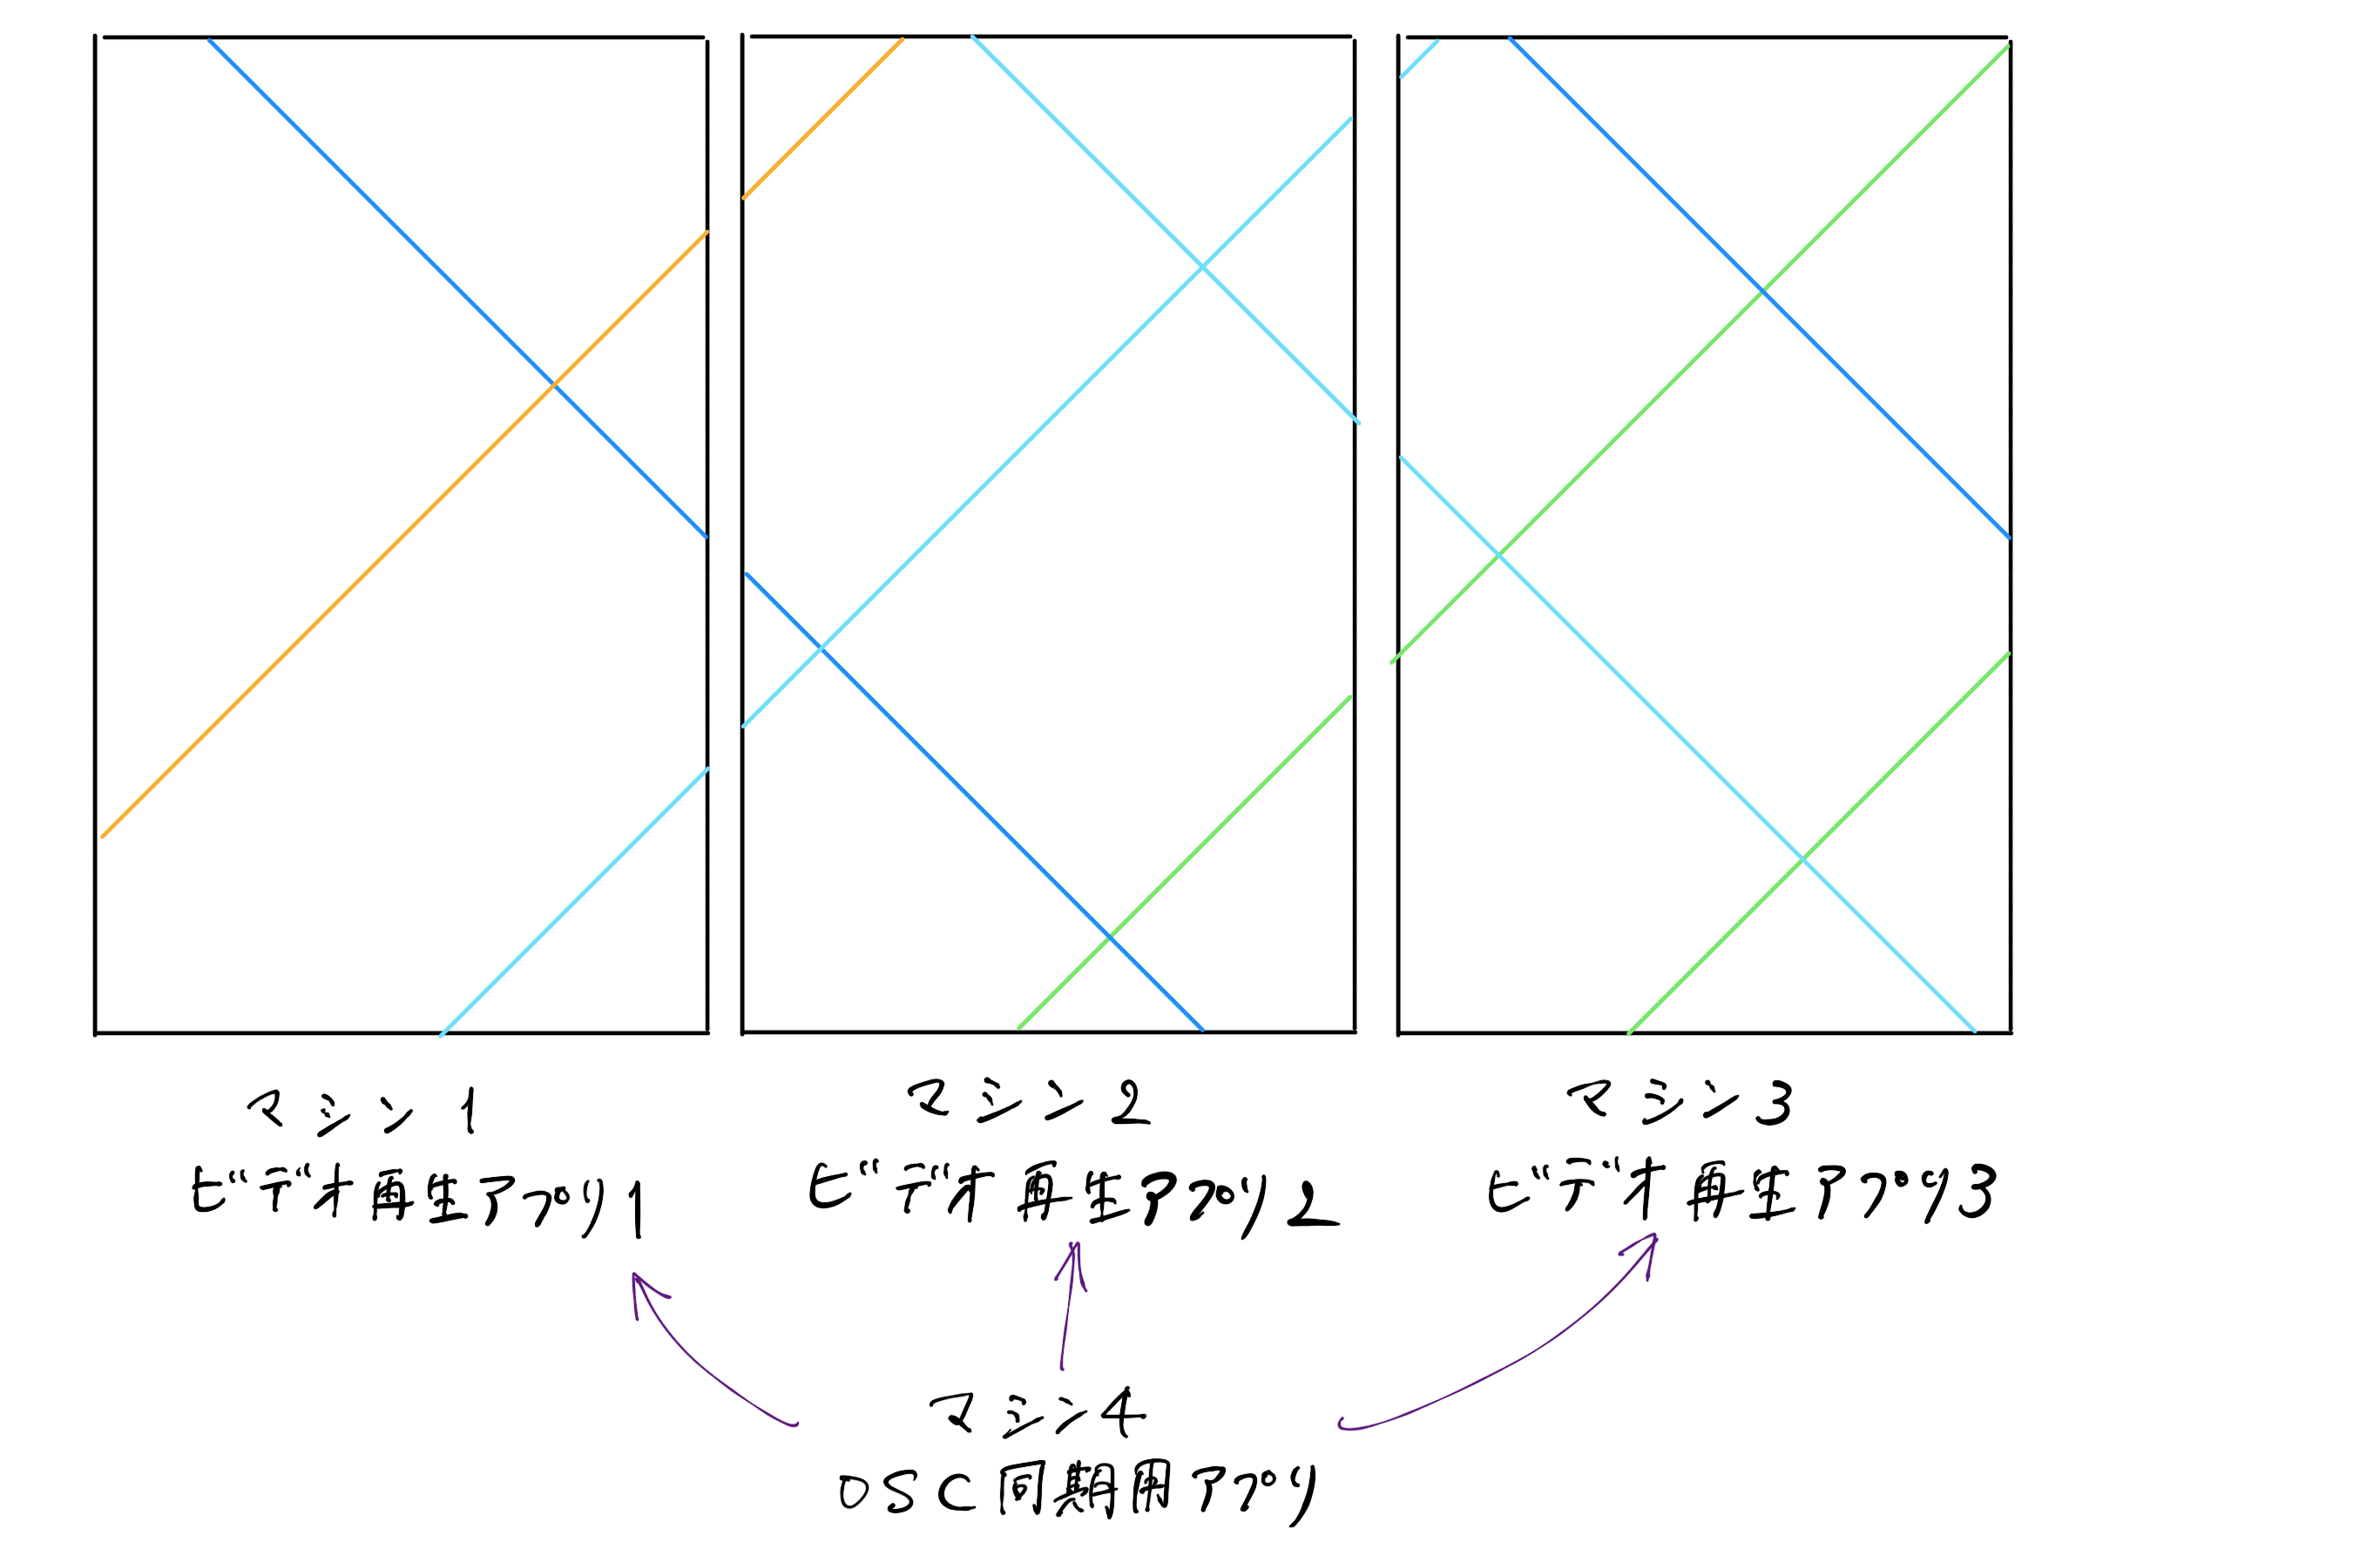
\includegraphics[width=100mm]{images/osc-1.png}
                    \caption{マシン間での映像同期参考図}
                    \label{fig:osc-1}
                \end{figure}
        \end{frame}

        \begin{frame}
            \frametitle{OSCの使用事例2 アプリ間で座標を渡す}
                \begin{figure}[htb]
                    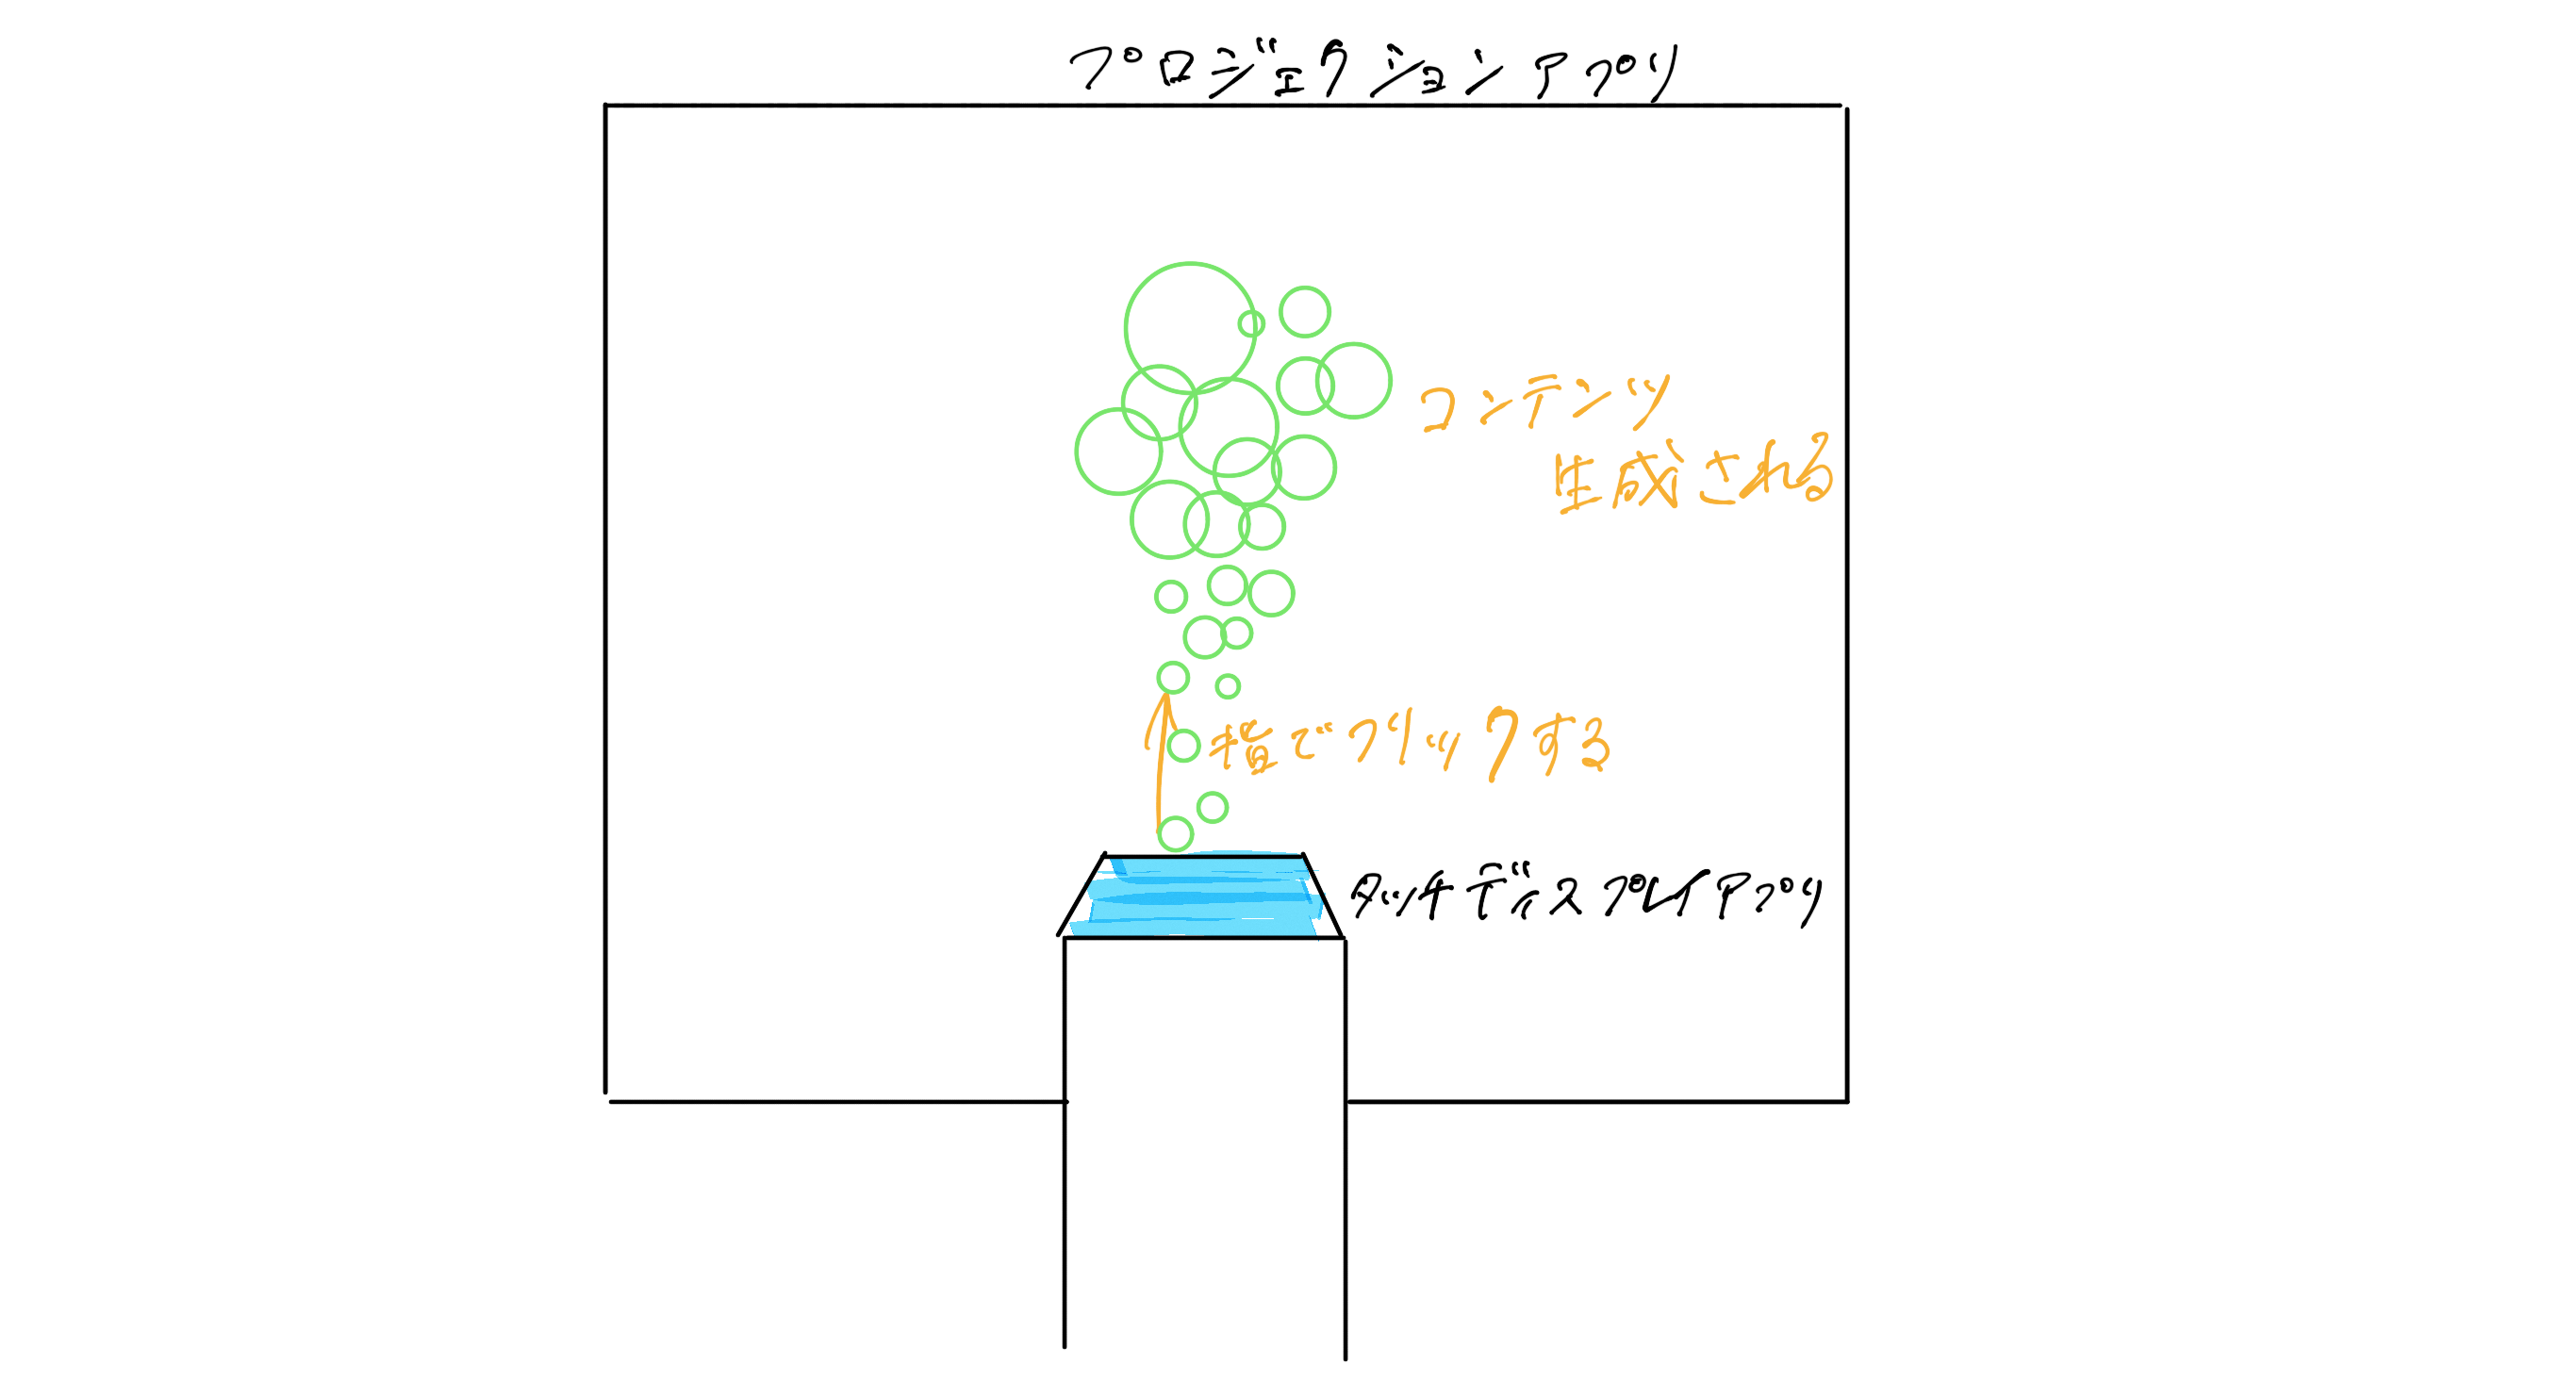
\includegraphics[width=100mm]{images/osc-2.png}
                    \caption{アプリ間で座標を渡す参考図}
                    \label{fig:osc-2}
                \end{figure}
        \end{frame}

        \begin{frame}
            \frametitle{oF - oF のOSC通信について}
            \begin{columns}[c]
                \begin{column}{0.80\textwidth}
                    \begin{block}{oF - oF のOSC通信に関しては以下にサンプルを公開しています}
                        \begin{itemize}
                            \scriptsize
                            \item 全体説明: http://scottallen.ws/tamabi/summerworkshop2017
                            \item プログラム: https://github.com/5c0tt411en/iddsummerworkshop2017
                            \item スライド: https://github.com/5c0tt411en/iddsummerworkshop2017/blob/master/Slide/day2
                        \end{itemize}
                    \end{block}
                \end{column}
            \end{columns}
        \end{frame}

    \subsection{信号のやりとり}
        \begin{frame}
            \frametitle{OSCを使った通信方法}
            \begin{block}{送信側}
                \begin{itemize}
                    \item 相手側マシンのipアドレスを指定: 169.254.11.14
                    \item 通信用ポートを指定: 8888
                    \item アドレスを指定: /stat
                    \item 型を明示して値を送信
                \end{itemize}
            \end{block}
            \begin{block}{受信側}
                \begin{itemize}
                    \item 通信用ポートを指定: 8888
                    \item 型を合わせて値を受信
                \end{itemize}
            \end{block}
        \end{frame}

    \subsection{touchOSC}
        \begin{frame}
            \frametitle{touchOSC}
            \begin{columns}[c]
                \begin{column}{0.50\textwidth}
                    \begin{figure}[htb]
                        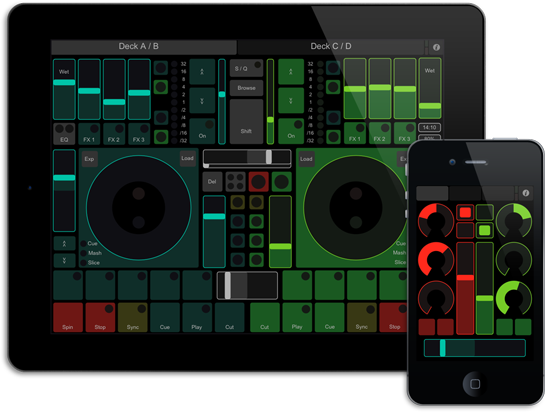
\includegraphics[height=40mm]{images/touch-1.png}
                        \caption{touchOSC画面(https://hexler.net/software/touchosc)}
                        \label{fig:touch-1}
                    \end{figure}
                \end{column}
                \begin{column}{0.50\textwidth}
                    \begin{block}{touchOSCの利点}
                        \begin{itemize}
                            \tiny
                            \item 手持ちのiOS, Androidがインターフェースになる
                            \item PCで自由にインターフェースを作成できる
                            \item iOSアプリを開発する必要がない
                            \item シンプルなので短時間でインターフェースが作成できる
                            \item コスト600円
                        \end{itemize}
                    \end{block}
                \end{column}
            \end{columns}
        \end{frame}

    \subsection{touchOSCからopenFrameworksへのOSC送信}
        \begin{frame}
            \frametitle{touchOSCを使ったコントロール}
                \tiny
                WS01/bin/touchOSC01.touchosc
                \begin{figure}[htb]
                    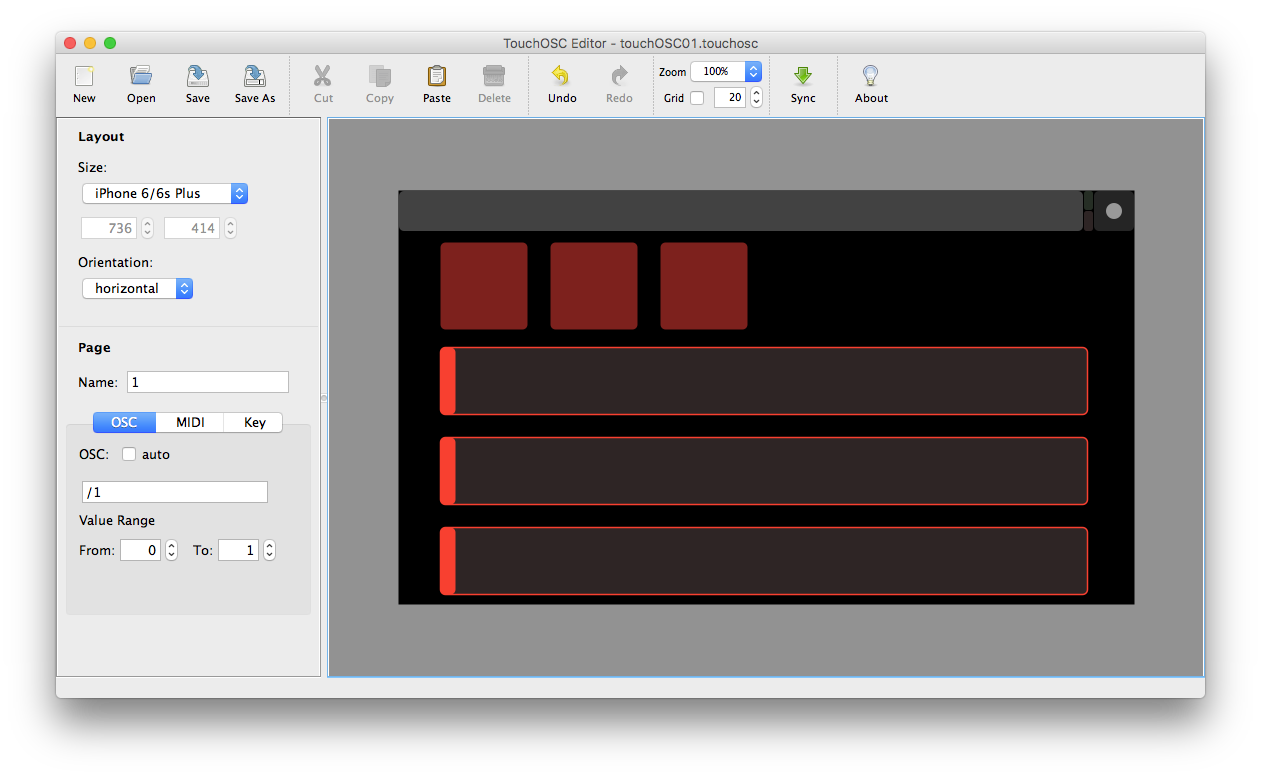
\includegraphics[width=100mm]{images/touch-2.png}
                    \caption{touchOSC01.touchosc 画面}
                    \label{fig:touch-2}
                \end{figure}
        \end{frame}

        \begin{frame}
            \frametitle{touchOSCを使ったコントロール}
                \tiny
                WS01/
                \begin{figure}[htb]
                    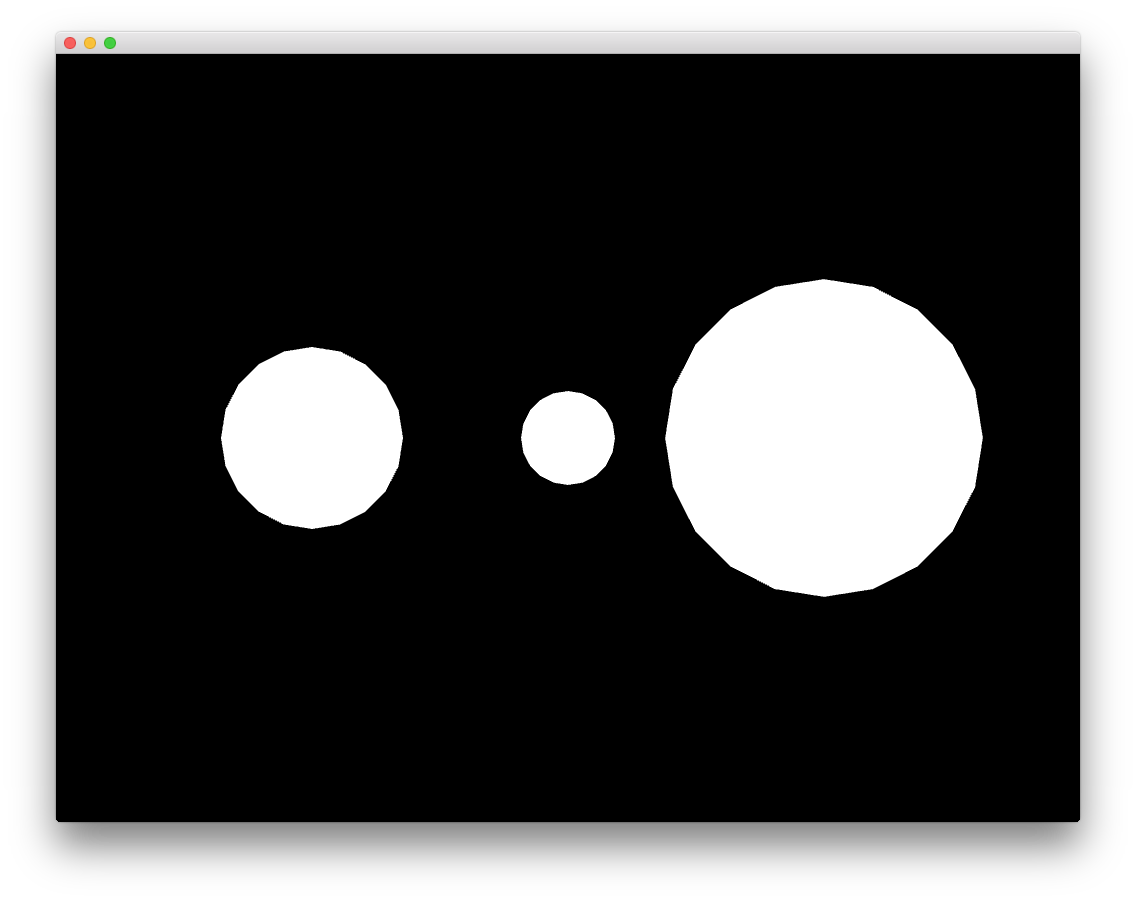
\includegraphics[width=75mm]{images/touch-3.png}
                    \caption{oF scene 1}
                    \label{fig:touch-3}
                \end{figure}
        \end{frame}

        \begin{frame}
            \frametitle{touchOSCを使ったコントロール}
                \tiny
                WS01/
                \begin{figure}[htb]
                    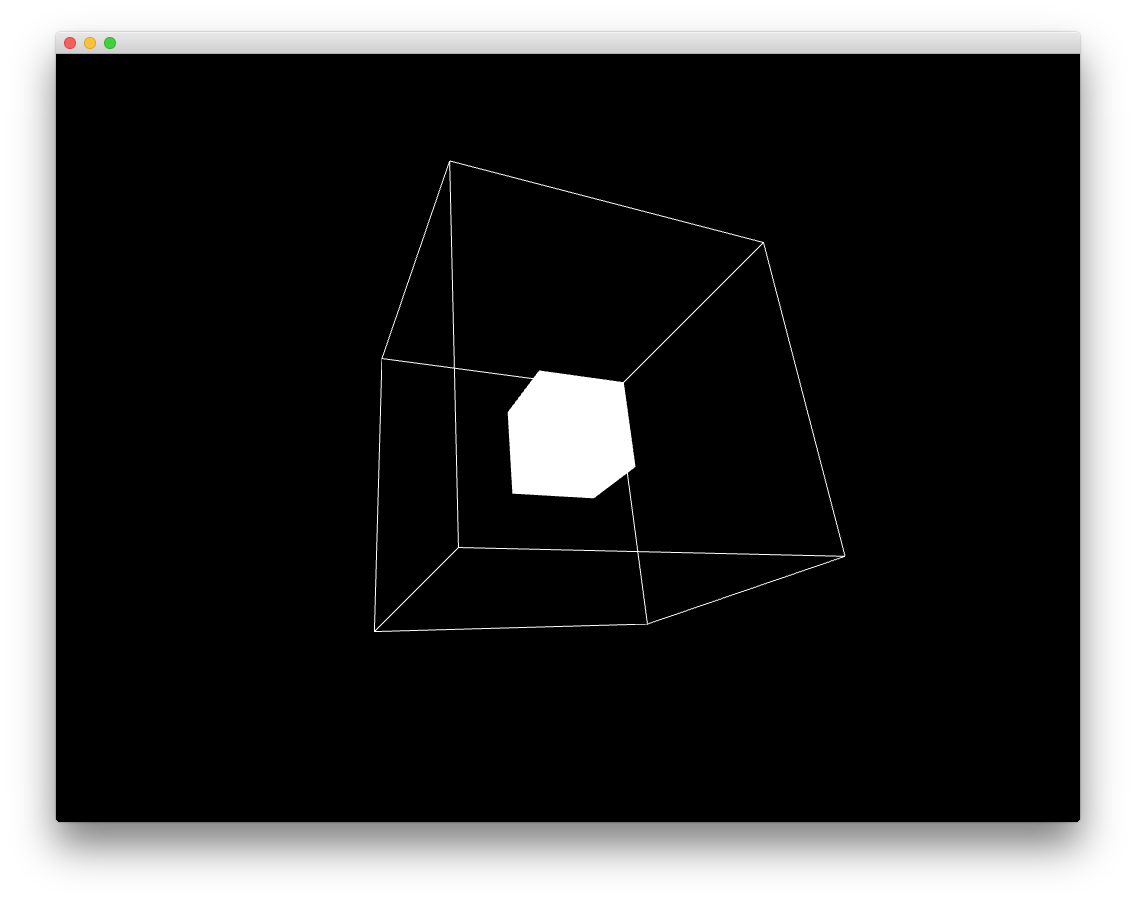
\includegraphics[width=75mm]{images/touch-4.png}
                    \caption{oF scene 2}
                    \label{fig:touch-4}
                \end{figure}
        \end{frame}

        \begin{frame}
            \frametitle{touchoscを使ったコントロール}
                \tiny
                WS01/
                \begin{figure}[htb]
                    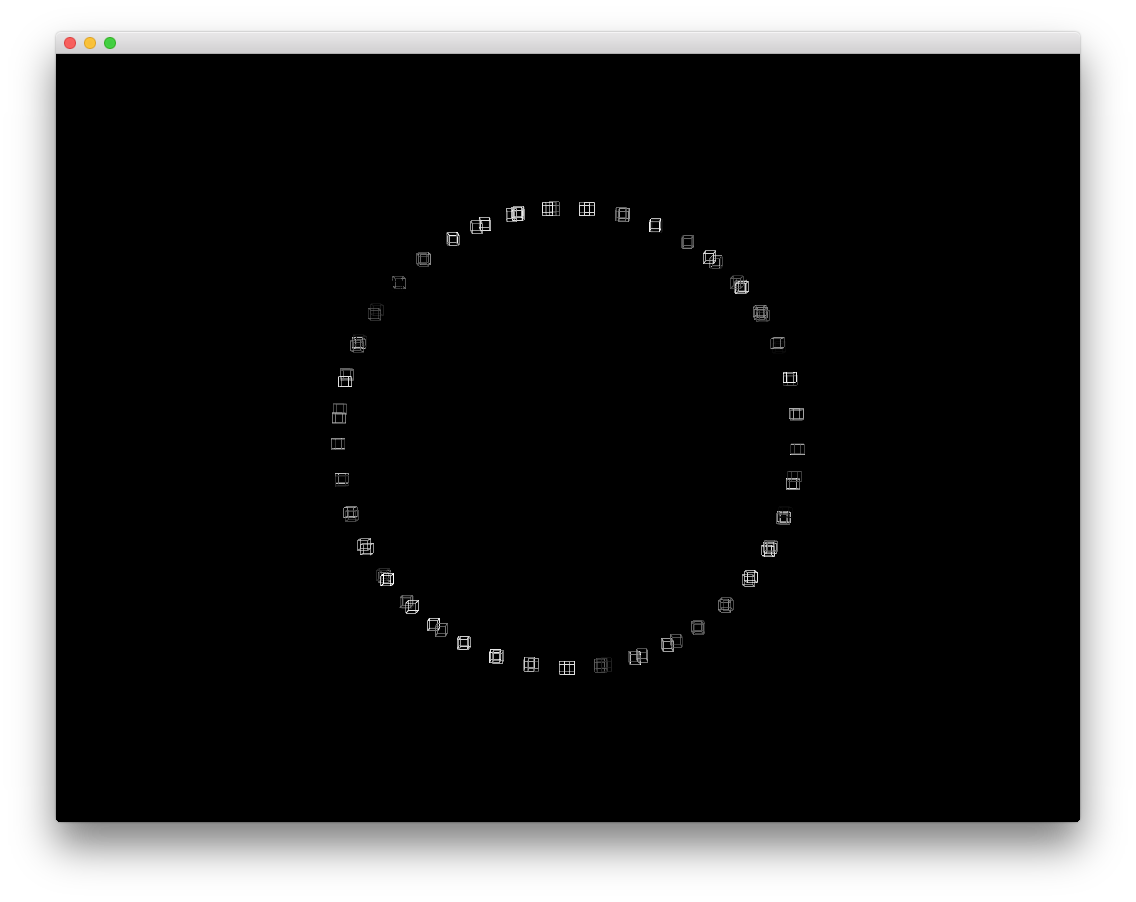
\includegraphics[width=75mm]{images/touch-5.png}
                    \caption{oF scene 3}
                    \label{fig:touch-5}
                \end{figure}
        \end{frame}

    \section{オーディオリアクティブ}
    \subsection{FFT}
        \begin{frame}
            \frametitle{FFTとは}
            \begin{block}{高速フーリエ変換(Fast Fourier Transform)の略 音の解析に使用される}
                \begin{itemize}
                    \item 音の高さ(周波数)ごとのレベルがわかる
                    \item サウンドビジュアライズが容易にできる
                    \item アルゴリズム自体は理解せずとも使用できる
                    \item GenerativeなVJは全員使っている
                \end{itemize}
            \end{block}
        \end{frame}

    \subsection{音を描画描画パラメータに割り当てる}
        \begin{frame}
            \frametitle{FFT 高速フーリエ変換 ofxEasyFft}
                \tiny
                WS02/
                \begin{figure}[htb]
                    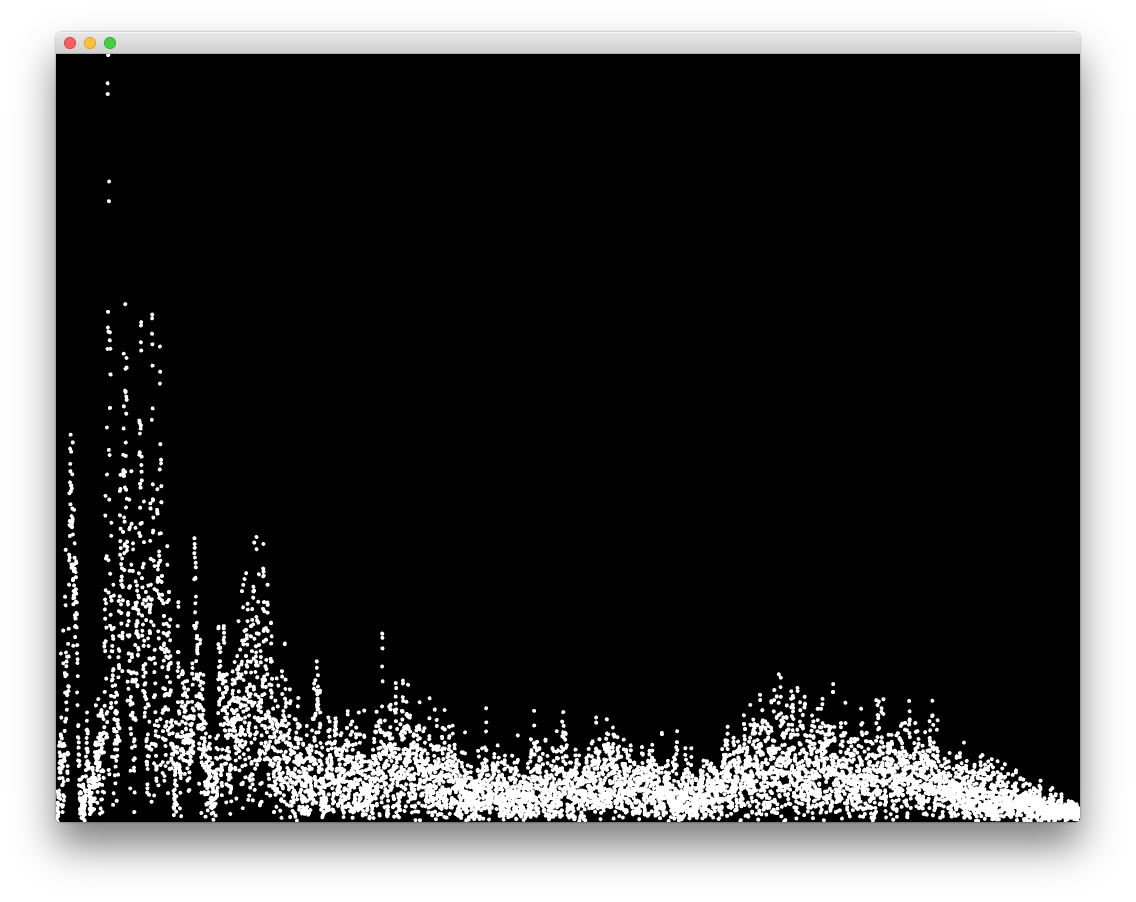
\includegraphics[width=75mm]{images/fft-1.png}
                    \caption{oF easyfft}
                    \label{fig:fft-1}
                \end{figure}
        \end{frame}

        \begin{frame}
            \frametitle{FFT 高速フーリエ変換 ofxProcessFft}
                \tiny
                WS03/
                \begin{figure}[htb]
                    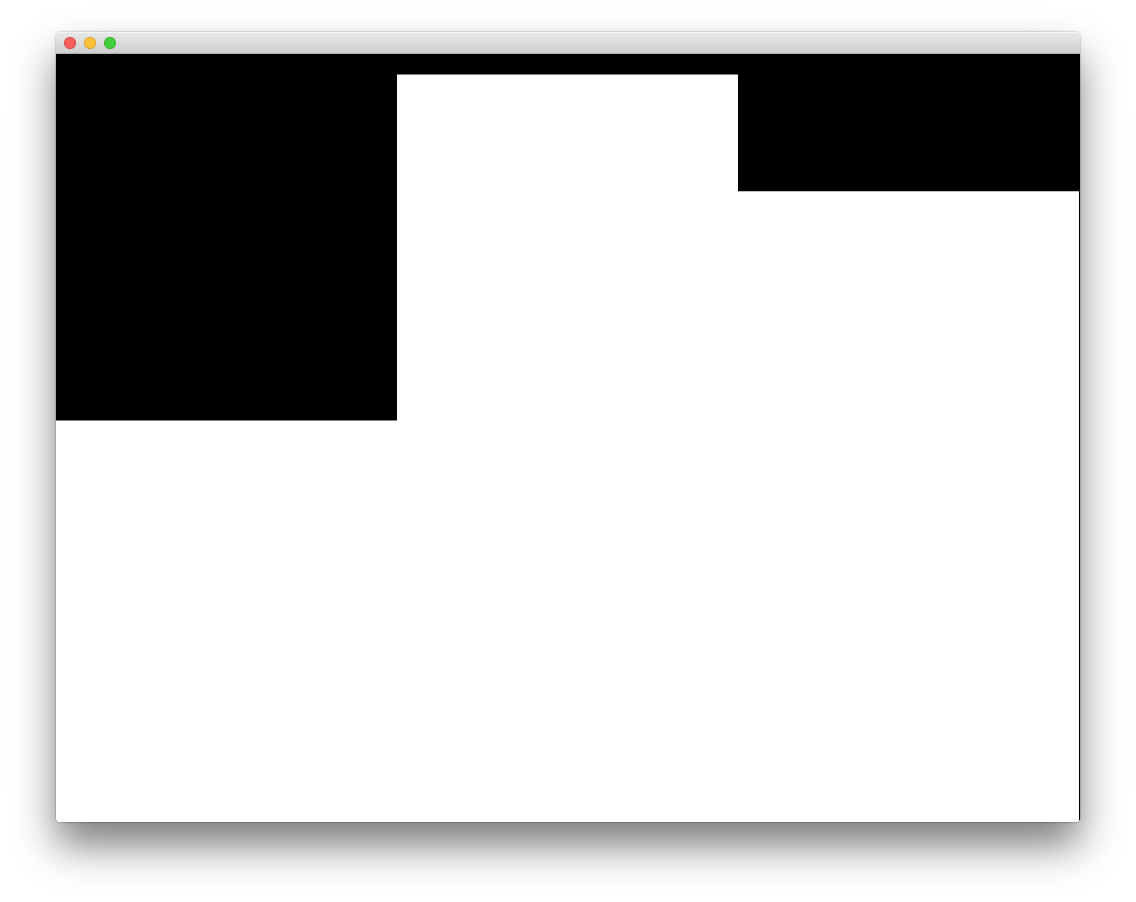
\includegraphics[width=75mm]{images/fft-2.png}
                    \caption{oF processfft}
                    \label{fig:fft-2}
                \end{figure}
        \end{frame}

    \subsection{しきい値を越えたら展開が進む}
        \begin{frame}
            \frametitle{FFT 高速フーリエ変換 ofxProcessFft}
                \tiny
                WS04/
                \begin{figure}[htb]
                    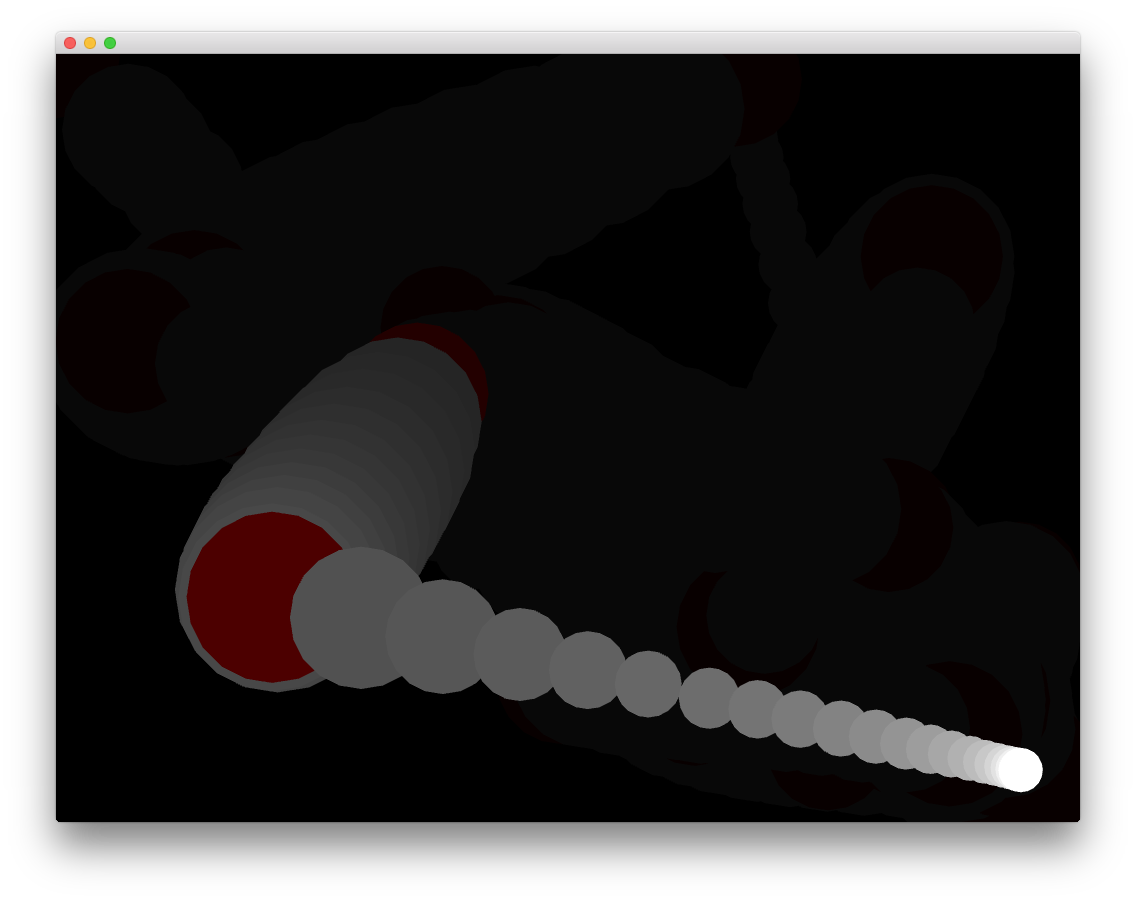
\includegraphics[width=75mm]{images/fft-3.png}
                    \caption{oF processfft}
                    \label{fig:fft-3}
                \end{figure}
        \end{frame}

        \begin{frame}
            \frametitle{FFT 高速フーリエ変換 ofxProcessFft}
                \tiny
                WS04/
                \begin{figure}[htb]
                    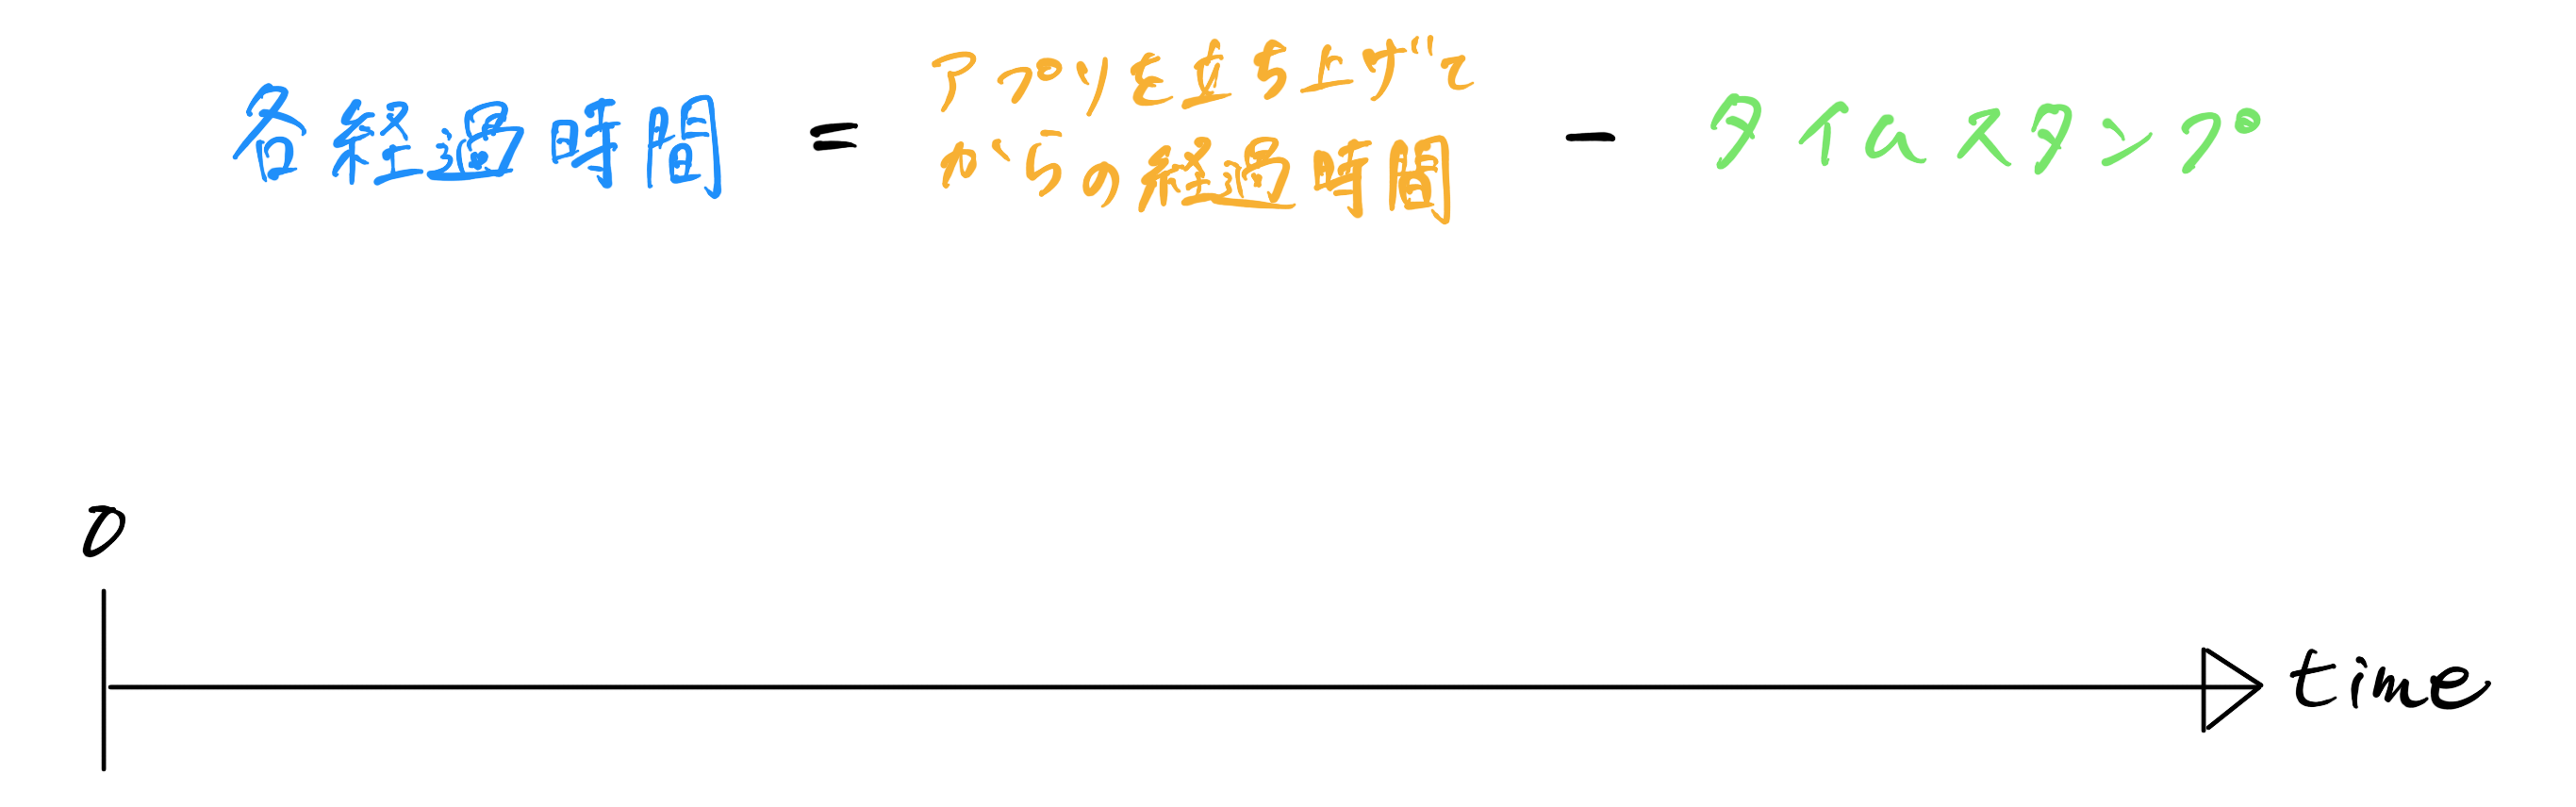
\includegraphics[width=100mm]{images/fft-4.png}
                    \caption{timeの考え方}
                    \label{fig:fft-4}
                \end{figure}
        \end{frame}

        \begin{frame}
            \frametitle{FFT 高速フーリエ変換 ofxProcessFft}
                \tiny
                WS04/
                \begin{figure}[htb]
                    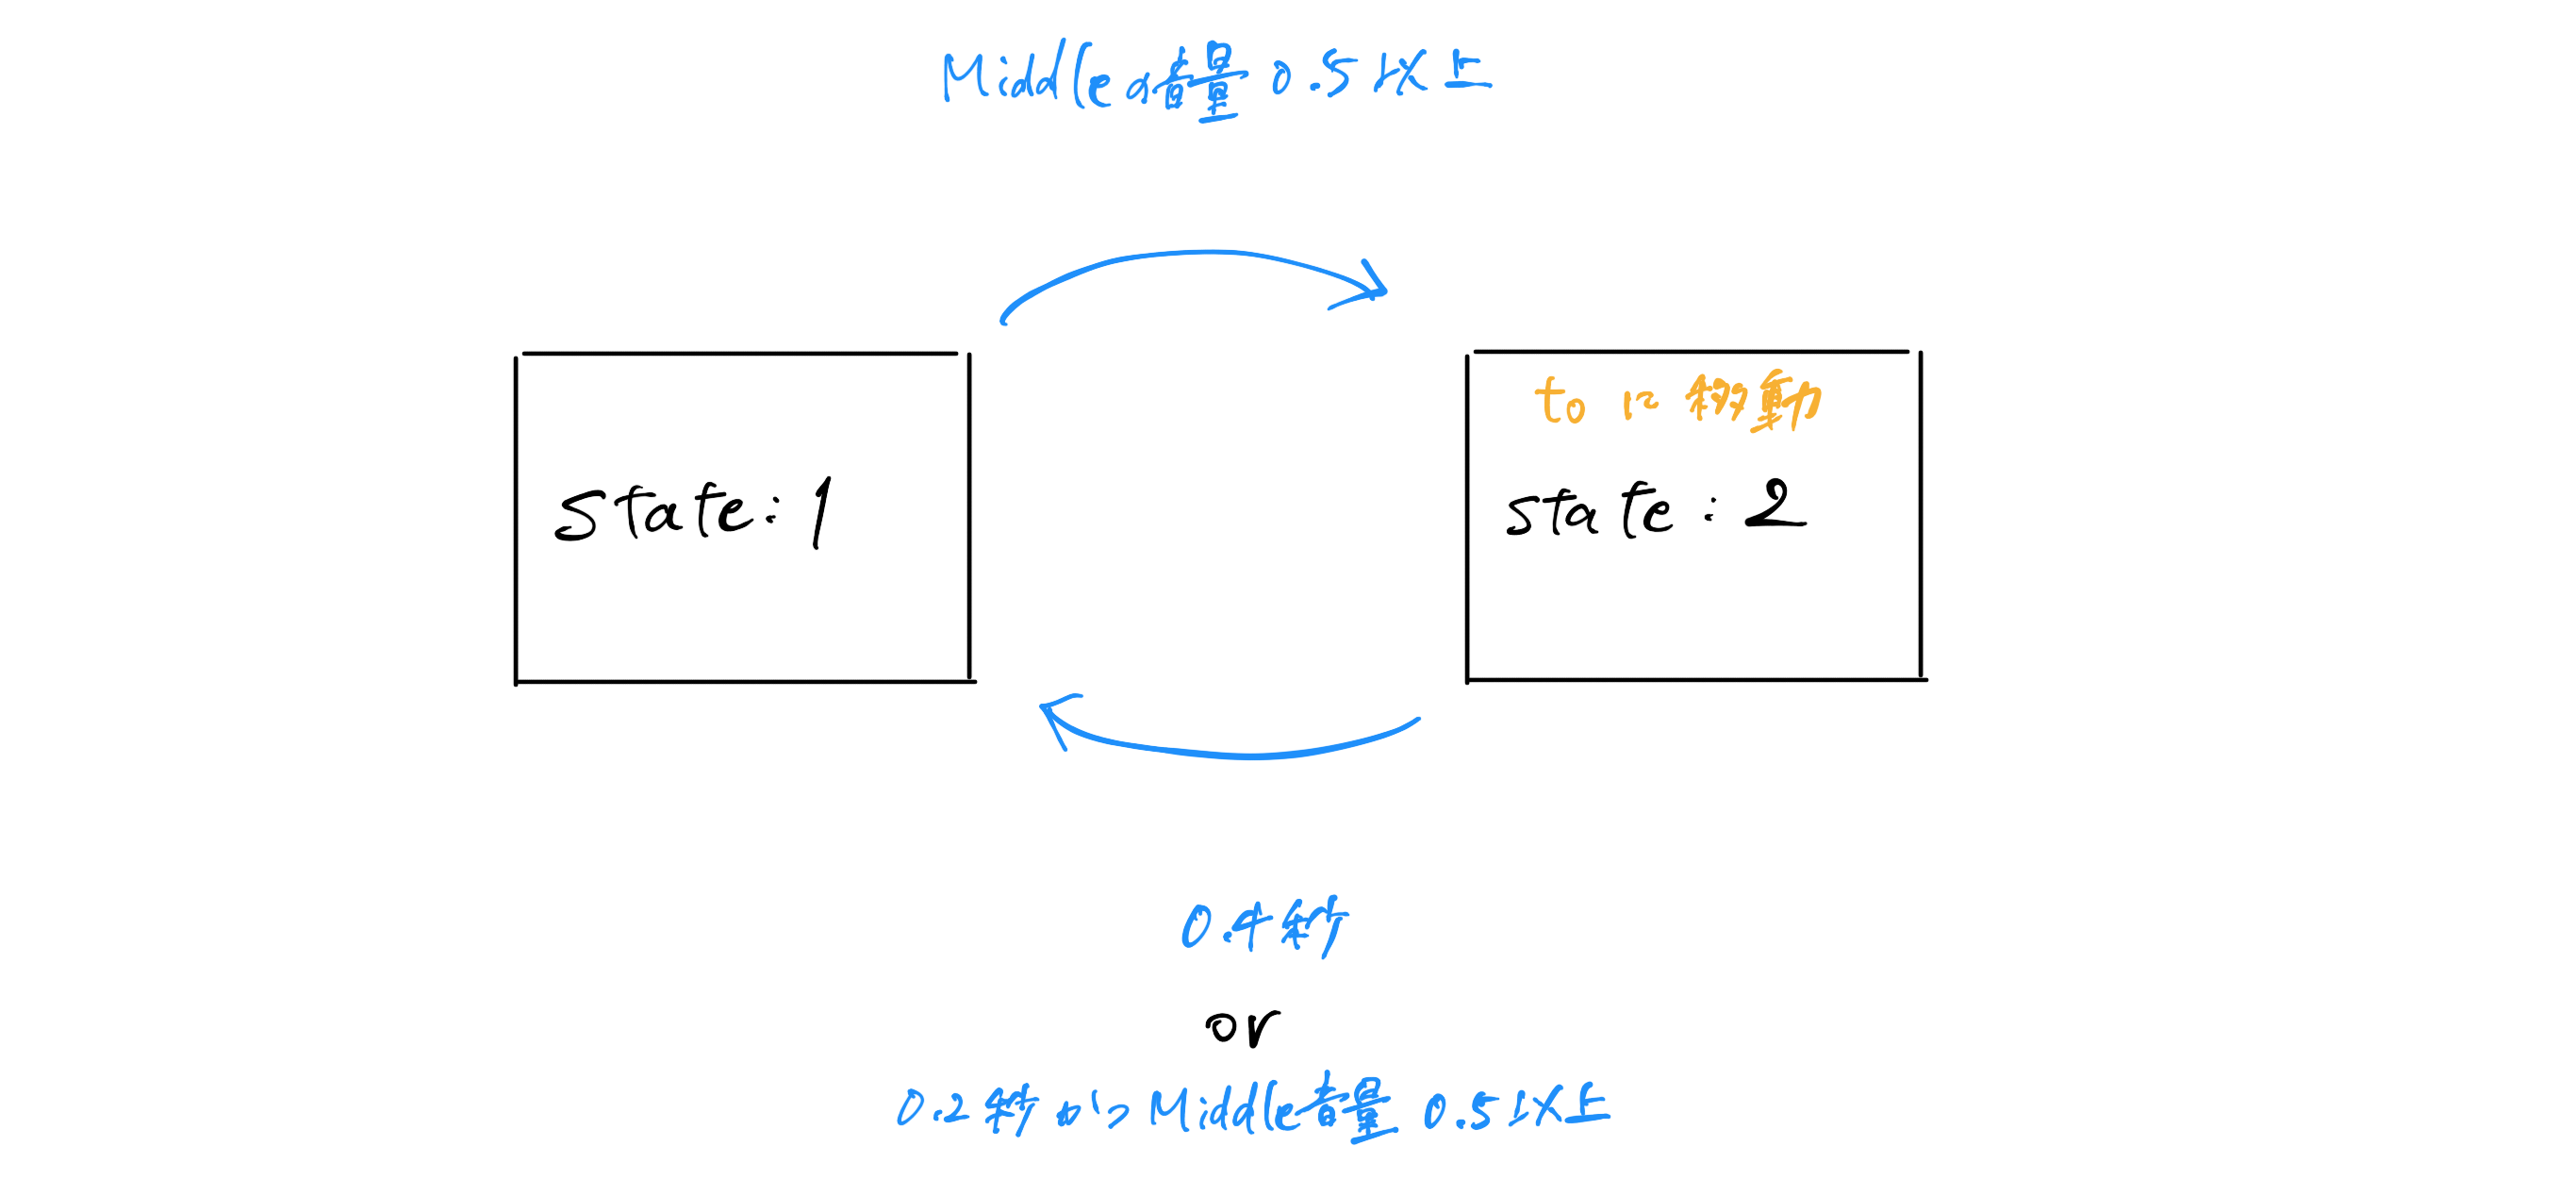
\includegraphics[width=100mm]{images/fft-5.png}
                    \caption{stateの移行図}
                    \label{fig:fft-5}
                \end{figure}
        \end{frame}

        \begin{frame}
            \frametitle{FFT 高速フーリエ変換 ofxProcessFft}
                \tiny
                WS04/
                \begin{figure}[htb]
                    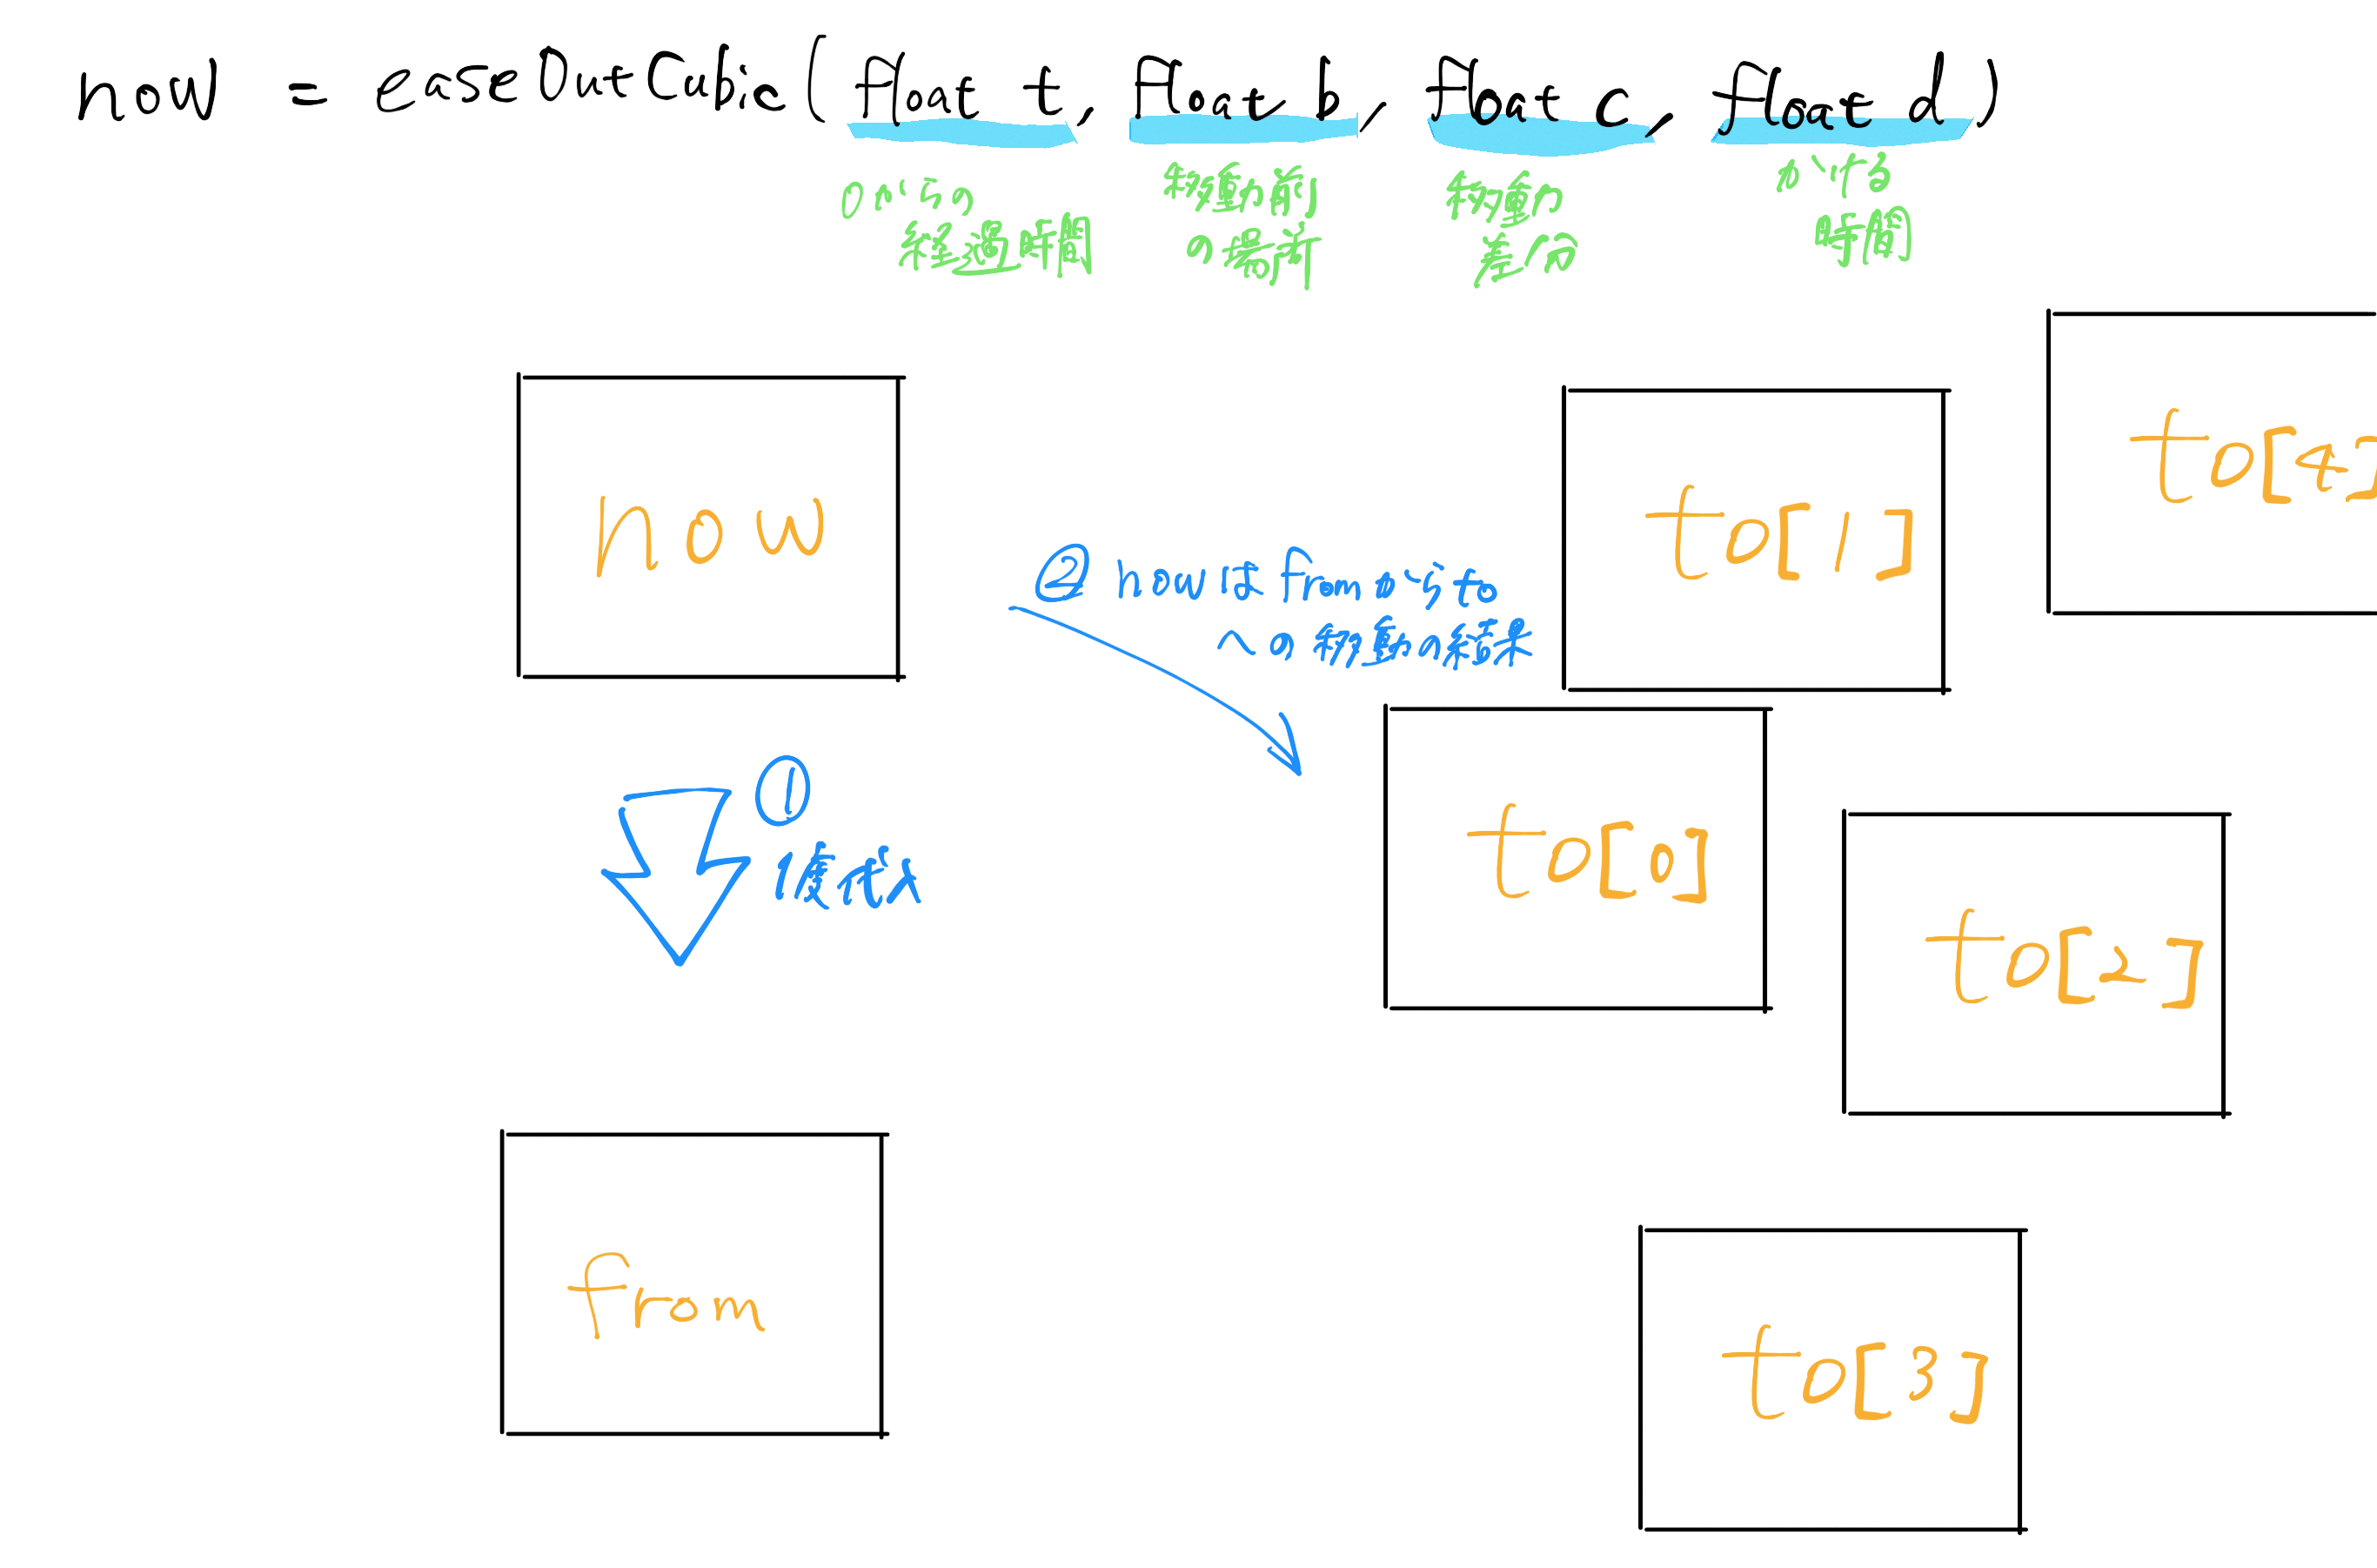
\includegraphics[width=80mm]{images/fft-6.png}
                    \caption{easing関数の考え方}
                    \label{fig:fft-6}
                \end{figure}
        \end{frame}
\end{document}

